%!TeX spellcheck = en-US
\documentclass[a4paper, 11pt]{article}
\usepackage[dvipsnames]{xcolor}
\usepackage[american]{babel}
\usepackage[utf8]{inputenc}
\usepackage[T1]{fontenc}
\usepackage[dvipsnames]{xcolor}
\usepackage{lmodern}
\usepackage{amssymb,amsmath}
\usepackage{comment} % enables the use of multi-line comments (\ifx \fi)
\usepackage{lipsum} %This package generates Lorem Ipsum filler text.
\usepackage{fullpage} % changes the margin
\usepackage{todonotes}
\usepackage{import}

\usepackage[backend=biber,bibstyle=authoryear,style=ieee]{biblatex}
\addbibresource{SingingBirds.bib}
\DeclareLanguageMapping{american}{american-apa}

\usepackage{xifthen}
\usepackage{soul}
\sethlcolor{Apricot}
\newcommand\bla[1]{\ifthenelse{\isempty{#1}}{\hl{**~bla~bla~**}}{\hl{**~#1~**}}}
\usepackage[unicode=true]{hyperref}
\usepackage[all]{hypcap} % ref link to the top of the figure

\usepackage{csquotes} % Dependency for APA


\hypersetup{breaklinks=true,
            pdfauthor={Paul Ecoffet},
            pdftitle={Report},
            colorlinks=true,
            citecolor=blue,
            urlcolor=blue,
            linkcolor=magenta,
            pdfborder={0 0 0}}
\urlstyle{same} % don't use monospace font for urls


\begin{document}
\noindent
\large\textbf{Présoutenance} \hfill \textbf{Paul Ecoffet} \\
\normalsize Cogmaster M2 \hfill Encadrants: Stéphane Doncieux, Benoît Girard \\
Tuteur: Mehdi Khamassi \hfill 20/01/17

\section*{Problem Statement}

The Zebra Finches are songbirds which learn the song of their tutor. They learn
it from 20 days post hatch (DPH) to 80 DPH \parencite{liu_juvenile_2004}. Their
learning can be split in three phases: i) they have a babbling phase from 20 DPH
to 40 DPH, then ii) a plastic song in which protosyllables from the tutor song
are produced then iii) a crystallized song at 80 DPH with a fixed song which is
a copy of the tutor's song. Zebra finches are commonly used as a model of speech
acquisition.

\textcite{deregnaucourt_how_2005} showed that sleep plays an important role in
the learning of tutor songs. Indeed, they showed that sleeping has a negative
impact on song restitution by zebra finches in the short term but a positive
impact on the long run. Indeed, song restitution is less complex and less
similar to the tutor song from one morning to the previous day evening, but the
greater this loss in performance was overall for one bird, the better this bird
will reproduce the tutor song at the end of its learning.
Figure~\ref{fig:sleep_performance} shows the negative impact on song similarity
the night has.

\begin{figure}[b]
  \center
  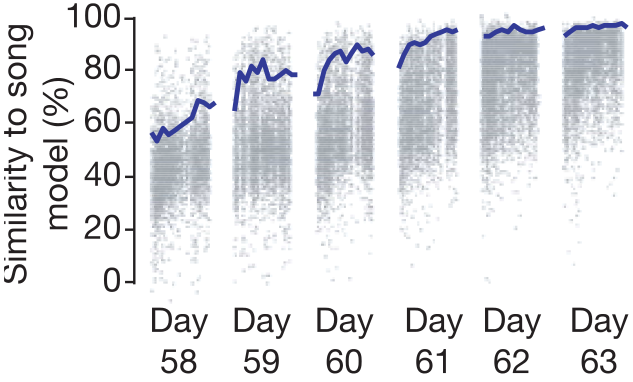
\includegraphics[width=0.5\linewidth]{media/deregnaucourt_sleep_performance.png}
  \caption{Song similarity from \textcite{deregnaucourt_how_2005}}
  \label{fig:sleep_performance}
\end{figure}

\textcite{dave_song_2000} has found replay sequences of neurones in the motor
cortex which correspond to their activity pattern when the birds sing in adult
zebra finches during their sleep. This shows that neurones that are highly
correlated with bird's own song (BOS) are activated during the night.

Our hypothesis is that during its sleep, the zebra finch restructures the
knowledge it has acquired so far. We hypothesize that this restructuring can
account for the loss of performance in the short term and an improvement of
performance in the long term.

The goal of this internship is to propose a model of the zebra finch song
learning which can explain different behavioral data observed such as the
correlation between the loss of performance every night and the overall
performance at the end of learning, and the different phases of bird song
learning (babbling, protosyllables, crystallized song).

\section*{Investigation/Research}

We want to build a model which is the most plausible in a real world environment
and which is biological plausible. To do so, we will use a bird song synthesizer
made by \textcite{boari_automatic_2015}. This synthesizer is a biophysical model
of zebra finch vocal apparatus. This synthesizer has the advantage that it be
parametrized with relatively few parameters to produce realistic bird songs. As
it models the zebra finch vocal apparatus, it is likely that the parameters we
send to this synthesizer must be similar to the instructions sent by the zebra
finch motor cortex to the vocal apparatus muscles. Indeed, the parameters for
this synthesizer is the the labia tension \(\alpha(t)\) and the air-sac pressure
\(\beta(t)\) in the apparatus.\todo{check alpha and beta that I keep mixing up}
\textcite{amador_elemental_2013, boari_automatic_2015} have managed to reproduce
zebra finches song using this synthesizer. The synthetic songs they produced
activated neurons in HVC which are highly selective to bird's own song (BOS).
This shows that the synthesized songs are accurate reproduction of BOS.

\textcite{amador_low_2014, boari_automatic_2015} have already found interesting
data by studying the parameters. Indeed, they have found that what can be seen
as syllable in the sensory space can be seen as one or several gestures in the
parameters space. Indeed, syllable are yield with continuous modification of the
parameters. A new syllable will trigger a huge discontinuity in the parameter
values.

\textcite{amador_elemental_2013} even claim to have found correlation with HVC
neuron spikes in zebra finches and the gesture trajectory extrema (beginning,
maximum, minimum and end) of these gestures. Though, very recent literature
shows that these correlates might have been untrue
\parencite{lynch_rhythmic_2016, picardo_population-level_2016}. Even though
there is no neural correlate with gesture trajectory extrema (GTE), we
hypothesize that GTE identification may play an important role in song learning,
as they signal changes in the progression of the parameters through time.

\section*{Proposed Solution}

Our goal is to design a simple hill climbing model (see
Fig.~\ref{fig:simple_model}) that fits one specific gesture and a gesture
identification algorithm. The gesture identification algorithm will try to
segment the tutor song in efficient gestures based on the bird current
knowledge. This two step algorithm is similar in some points to an
Expectation-Maximization algorithm \parencite{dempster_maximum_1977}.

So as to do a first gesture segmentation, we will use motor babbling so that the
bird robot can explore its sensorimotor space and segment the tutor song based
on its babbling. We will then use a interest model to choose which syllable to
train \parencite{baranes_active_2013}. The overview of the whole algorithm is
shown in Figure~\ref{fig:goal_def}. Our idea is that the maximization of the
identified gestures occurs during the day and explain the overall advancement
in performance.

This part will only cover the learning of gesture, but not the linkage between
these gestures. We have yet to find how to learn the pattern of the syllables
and the song. This algorithm should be able to use in a smart way the knowledge
built by the gesture learning system. The algorithm that learn the syllable
transition should also be able to reproduce the different learning strategies
that a zebra finch can have. Indeed, the zebra finch can either have a serial
strategy, where it only learn one specific syllable at a time, or have a motif
strategy, where it learn to reproduce the whole tutor song at every try.

\begin{figure}[tb]
\centering{
\def\svgwidth{0.9\linewidth}
\import{media/}{simple_process_schema.pdf_tex}
\caption{Simple hill climbing model \label{fig:simple_model}}
}
\end{figure}
\begin{figure}[tb]
\centering{
\def\svgwidth{0.8\linewidth}
\import{media/}{goal_def_schema.pdf_tex}
\caption{Define goals based on knowledge \label{fig:goal_def}}
}
\end{figure}

\section*{Expected Implementation}

The learning algorithm that we want to suggest must be biologically plausible,
therefore we will use the Song Synthesizer from \textcite{boari_automatic_2015}
to generate real sound-waves. We have already implemented the Python binder to
the compiled synthesizer. These sound-waves will then be processed by an
auditory system. We plan at first to use Mel-Frequency Cepstrum Coefficients
(MFCC), which are used in speech recognition for Humans.
\textcite{chou_studies_2008} showed that MFCC can be used to classify birdsongs.
MFCC sums up audio signal in a few coefficients per time window. Though, we
obtained strange results using MFCC squared error between the real song and our
generated bird song. Indeed, even though our generated bird songs were
qualitatively very bad as they sound like white noise, the difference between
their MFCC differences with the real song were lower than the generated song by
\textcite{boari_automatic_2015} which sound qualitatively very similar. We are
currently trying to fine tune the use we have of MFCC and get a better
understanding of their behavior. We may change for another sound representation.
As the exact length of a syllable may vary from try to try, we plan to use
Dynamic Time Warping (DTW) algorithm to avoid error accumulation for a slightly
off-time syllable. MFCC and DTW used together are powerful tools for speech
recognition \parencite{muda_voice_2010}.

We plan to use a Nearest-Neighbor algorithm to hill climb toward the goals the
algorithm defines and remember each try it makes so as to define more realizable
goals. The Nearest-Neighbor algorithm and the interest model are available
through the Explauto python module \parencite{moulin-frier_explauto:_2014}.

\section*{Analysis \& Testing}

To assess the quality of our model, we have selected several criteria to meet.
First, we want our algorithm to reproduce the results from
\textcite{deregnaucourt_how_2005}. This include observing the increase of song
similarity (a measure defined by \textcite{tchernichovski_procedure_2000}) over
the development of the bird, that the song similarity decrease over night, but
that this decrease is positively correlated with the song restitution at the end
of the learning. To do that, we will use the same statistical test that
\textcite{deregnaucourt_how_2005} have done on the same set of features. We will
therefore use

Then, we expect our model to yield at first protosyllables, then syllables and
go into the crystallized song. \todo{look at how I can evaluate this by
clustering}

Finally, we want that our algorithm identify the same amount of GTE per second
that are identified by \textcite{boari_automatic_2015}.

\section*{Final Evaluation}

The goal of building this model is being able to build new hypotheses that can
be tested in behavioral or neurobiological experiment on the zebra finch. Once
the model is fully working and respond to our expectations in reproducing the
literature, we will study its behaviors so as to design new hypotheses.

\printbibliography{}

\end{document}
